\chapter{Data Analysis} \label{ch:analysis}
The availabe spectra were extrapolated to calculate the transverse energies and charged particle multiplicities. Details follow.

\subsection{STAR $p_{T}$ spectra}
This thesis details the method of transverse energy analysis through the use of $p_{T}$ spectra from the STAR BES data. As described in section \ref{subsec:tracking_STAR}, the TPCs and TOF detectors in STAR can identify particles as well as their trajectories and ultimately measure their multiplicity distributions with respect to the momenta. \citet{PhysRevC.96.044904} reports the results for the $p_{T}$ spectra for six different identified hadrons, $\pi^+$, $\pi^-$, $K^+$, $K^-$, $p$, and $\bar{p}$, from the STAR experiment. The spectra come from $\sqrt{s_{NN}}$ = 7.7, 11.5, and 39 GeV Au+Au collisions data taken in the year 2010, and from $\sqrt{s_{NN}}$ = 19.6 and 27 GeV Au+Au collisions data taken in 2011, both as part of the BES Program. Figure \ref{fig:BESPaper_pTSpectra} \cite{PhysRevC.96.044904} shows the spectra corresponding to 39 GeV collisions categorized into seven different collision centralitiy classes. Additionaly, preliminary spectra were available from the STAR experiment for idenfitied lambdas and anti-lambdas. All of these spectra were used to calculate an estimate of the total transverse energy per event per particle species. This result was then used to estimate the total transverse energy due to all the collision products.
\begin{figure}[h]
  \centering
  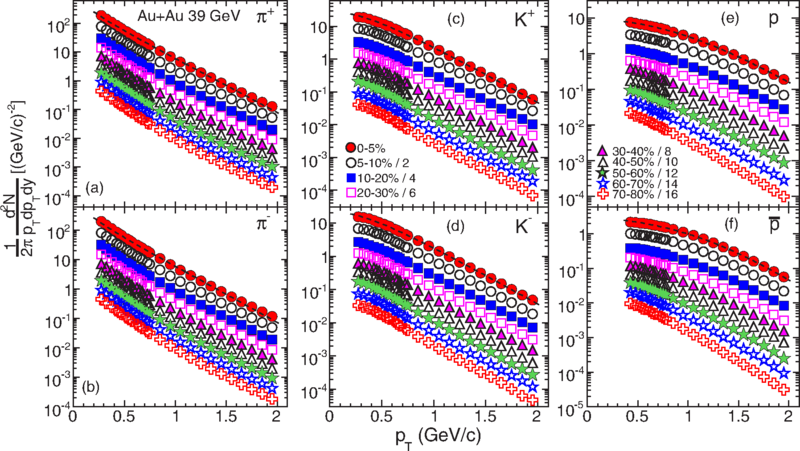
\includegraphics[width=6.5in]{../figures/PhysRevC-96-044904_pTSpectra_39.png}\\
  \caption{Transverse momentum spectra for $\pi^{+}$, $\pi^{-}$, $K^+$, $K^{-}$, $p$, and $\bar{p}$ at midrapidity ($|y|$ $<$ 0.1) from 39 GeV Au+Au collisions at RHIC. The fitting curves on the 0-5\% central collision spectra for pions, kaons, and protons/anti-protons represent, respectively, the Bose-Einstein, $m_{T}$-exponential, and double-exponential functions \cite{PhysRevC.96.044904}.}\label{fig:BESPaper_pTSpectra}
\end{figure}

The corrections applied by \citet{PhysRevC.96.044904} to the raw data to obtain the spectra and the reported systematic uncertainties in their results are discussed below (under construction)
.....................................................................................................

\section{Extrapolation of Spectra}
The available spectra were limited to a range of transverse momenta from around 0.25 GeV/c to around 2 GeV/c (for pions). To account for the transverse energy corresponding to the momenta for which there was no available data, an extrapolation had to be used. The model used for the extrapolation and the associated statistics are discussed below.

\subsection{Boltzmann-Gibbs Blast Wave}
The blast wave is a common model used in the analysis of the particle spectra [refs 4, 43 and 51 from PhysRevC.96.044904]. The specific model used in this thesis is the Boltzmann-Gibbs blast wave (BGBW) as represented in equation \ref{eqn:bgbw}. It has the parameters mass, temperature, beta, v, and n. I assume that any anomalies in the magnitude of the normalization parameter do not affect the results significantly insomuch as they don't lead to: 

(a) unreasonable relative errors in the extrapolated values of the transverse energy,

(b) any of the spectral fits having the extrapolated transverse energy more than that calculated from just the available spectra, and

(c) for the 200 GeV collision samples, at least, the extrapolation at higher $p_{T}$ being more than that at lower $p_{T}$.

	\begin{equation}\label{eqn:BGBW}
	BGBW
	\end{equation}

\subsection{Fitting Spectra to BGBW}
Figure \ref{fig:fit} presents an example of a Boltzmann-Gibbs Blast Wave (BGBW) fit on one of the individual particle spectra with $\chi^{2}$/n.d.f as well as other statistics and the associated errors. A parallel-coordinates plot is presented in the next chapter in fig. \ref{fig:parallelCoord}, which shows the measured centralities, two of the good-fit parameters, and the calculated transverse energies for 270 different particles (lambdas not included).

	\begin{figure}[h]
	  \centering
	  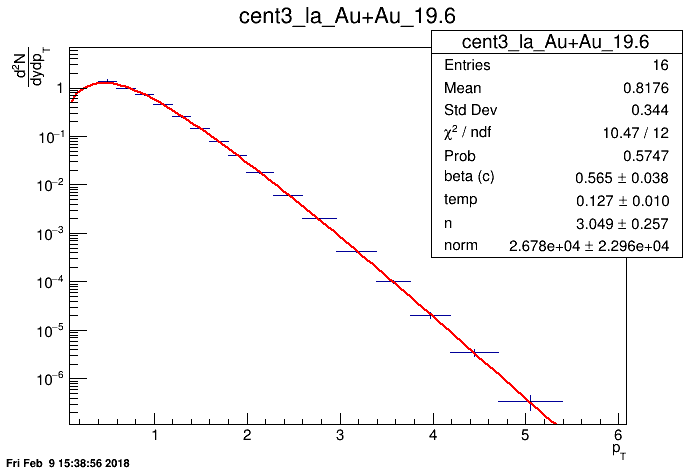
\includegraphics[width=4.5in]{figures/cent3_la_Au+Au_196.png}
	  \caption{Red curve shows the Boltzmann-Gibbs blast wave functional fit on the PRELIMINARY transverse momentum spectrum for lambda particles identified by the STAR detector for 19.6 GeV Au+Au collisions (10-15\% central). Parameters extracted from the chi-square goodness-of-fit test, as well as other statistics, are shown in the box on the top right.}\label{fig:fit}
	\end{figure}

\section{Calculations from the Spectral Fits}
\subsection{Calculation of $\frac{dE_{T}}{dy}$, $\frac{dE_{T}}{d\eta}$, $\frac{dN_{ch}}{dy}$, and $\frac{dN_{ch}}{d\eta}$}
\subsection{Corrections for Unidentified Particles and Estimation of Total $E_{T}$}\label{corrections}
It is reasonable to assume that, at high energies, there should be roughly the same multiplicity of all the isospin states of a final state particle. Table \ref{table:isospinStates} lists the isospin states associated with the pion, the kaon, the proton, and the lambda particles.

	\begin{table}[h!]
	\centering
	\begin{tabular}{|c c|}
	%\tabletypesize{\scriptsize}
	%\rotate
	\hline
	Particle & Isospin multiplets \\ [0.5ex]
	\hline
	\hline
	pion & $\pi^{+}, \pi^{0}, \pi^{-} $ \\
	kaon & $K^{+}, K^{0}, K^{-}, \bar{K}^{0}$ \\
	proton & $p, n, \bar{p}, \bar{n}$  \\
	lambda & $\Lambda, \bar{\Lambda}$  \\ [1ex]
	\hline
	\end{tabular}
	\caption{Isospin states of different identified particles.}
	\label{table:isospinStates}
	\end{table}
	
	.............text content.............
	
	\begin{equation}\label{eqn:TotET}
	E_{T} = 3E_{T}^{\pi} + 4E_{T}^{K} + 4E_{T}^{p} + 2E_{T}^{\Lambda}
	\end{equation}
	
 ................text content...................
 
\subsection{Lambdas Centralitiy Adjustments and $E_{T}$ Interpolations}
The centrality bins corresponding to the lambdas spectra were slightly different from those corresponding to the rest of the particles........
%\subsection{}
\section{Uncertainties}
......... 100\% correlated point-to-point and uncorrelated between particles........ ?
%\section{}
